\documentclass{beamer}
\usepackage[english, russian]{babel}
\usetheme{Boadilla}

\title{GraphSASRec}
\author{@matfu21}

\begin{document}

\frame{
\frametitle{GraphSASRec}
\begin{columns}[onlytextwidth,T]
  \column{\dimexpr\linewidth-43mm-5mm}

  Ideas:
    \begin{enumerate}
      \item[*] Improve next item prediction task with topological information.
    \end{enumerate}
  Method:
    \begin{enumerate}
      \item[*] Build heterogeneous graph.
      \item[*] Learn complex graph representations of items in heterogeneous network.
      \item[*] Link-prediction loss: $$-\sum_{e \in G} (log \sigma (f(e)) +$$ 
      $$ + \sum_{e' \in N(e)} \log \sigma(1 - f(e')))$$.
      \item[*] Reuse freeze graph vectors in SASRec.
    \end{enumerate} 

    \column{150mm}

    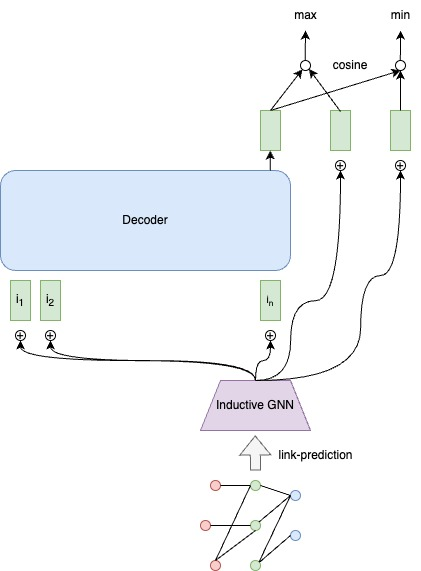
\includegraphics[width=50mm]{graphsasrec.jpg}
\end{columns}
}

\end{document}